\documentclass{beamer}
\usepackage[utf8]{inputenc} % remplace utf8 con latin1
                            % si va a compilar en un sistema
                            % Windows
\usepackage{hyperref}
\usepackage[spanish]{babel}
\usepackage{multicol}
\usepackage{graphicx}

% Agregamos información del autor y titulo

\title{Ejemplo en Beamer}
\author{David Raygoza Gómez}
\date{5 de Diciembre del 2018}

\begin{document}

\begin{frame}
	\titlepage
\end{frame}

\begin{frame}
	Este es un ejemplo basico en beamer, el paquete para generar presentaciones en \LaTeX.
\end{frame}

\begin{frame}
	Las instruciones \emph{ \textbackslash begin\{frame\} } y \emph{\textbackslash  end\{frame\}} delimitan lo que aparecera en una diapositiva, podemos usar cualquier instrucción de \LaTeX sin problemas.
\end{frame}

\begin{frame}
	
	Como lo es poner figuras.
	
	\begin{figure}
		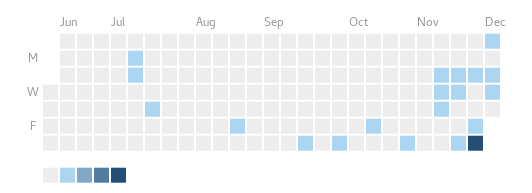
\includegraphics[scale=0.2]{imagenes/actividad.png}
		\caption{Actividad}
		\label{img_1}
	\end{figure}

	Cambiando su tamaño con [scale=escala]

	\begin{figure}
		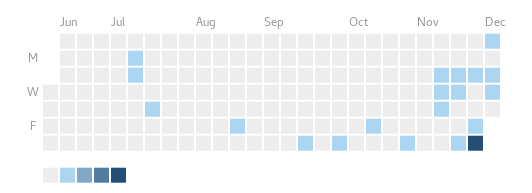
\includegraphics[scale=0.1]{imagenes/actividad.png}
		\caption{La misma imagen a la mitad de la escala}
		\label{img_2}
	\end{figure}
	
	Teniendo cuidado de que sean del tamaño adecuado, o no cabra en la diapositiva.
	
\end{frame}

\begin{frame}
	Listas
	
	\begin{enumerate}
		\item Elemento 1
		\item Elemento 2
		\item Elemento 3
	\end{enumerate}

	\begin{itemize}
		\item Un elemento
		\item Otro elemento
		\item Algo mas
	\end{itemize}

	Como con las imagenes recuerde no pasarse de lo que quepa en la diapositiva,
	
\end{frame}

\begin{frame}
	Aunque podemos usar \emph{multicols} para automaticamente mostrar la lista en varias columnas y que asi quepan.

	\begin{multicols}{3}
		\begin{enumerate}
			\item Elemento 1
			\item Elemento 2
			\item Elemento 3
			\item Elemento 4
			\item Elemento 5
			\item Elemento 6
			\item Elemento 7
			\item Elemento 8
			\item Elemento 9
			\item Elemento 10
			\item Elemento 11
			\item Elemento 12
			\item Elemento 13
			\item Elemento 14
			\item Elemento 15
			\item Elemento 16
			\item Elemento 17
			\item Elemento 18
			\item Elemento 19
			\item Elemento 20
		\end{enumerate}
	\end{multicols}


\end{frame}

Y usar \emph{resizebox} para evitar que las tablas se salgan de la diapositiva.

\begin{table}
	\centering
	\resizebox{10cm}{!} {
	\begin{tabular}{|c|c|c|c|c|c|c|c|c|}
	\hline
	\multicolumn{5}{|c|}{Puerto fuente} & \multicolumn{4}{|c|}{Puerto destino} \\ \hline
	\multicolumn{9}{|c|}{Numero de secuencia} \\ \hline
	\multicolumn{9}{|c|}{Numero de reconocimiento} \\ \hline
	Longitud cabecera & Reservado & URG & ACK & PSH & RST & SYN & FIN & Tamaño ventana \\ \hline
	\multicolumn{5}{|c|}{Suma verificación} & \multicolumn{4}{|c|}{Puntero a datos urgentes} \\ \hline
	\multicolumn{9}{|c|}{Opciones} \\ \hline
	\multicolumn{9}{|c|}{Datos} \\ \hline
	\end{tabular}
	}
	\caption{Tabla Ejemplo.}
	\label{c2_tabla_segento_tcp}
	\end{table}

\begin{frame}
	\begin{center}
		Tambien puede centrar elementos con ayuda de \emph{center}
	\end{center}	
\end{frame}

\begin{frame}
	Y referencias figuras, como la Figura \ref{img_1} o a la tabla \ref{c2_tabla_segento_tcp} con ayuda de  \emph{\textbackslash ref}
\end{frame}

\end{document}
